
\documentclass[ms.tex]{subfiles} 
\begin{document} 

\section{Methods} 
\label{sec:methods} 

\begin{itemize} 
	\item Since we wish to test the impact of various assumptions about 
	nucleosynthetic yields while taking into account stellar migration, 
	multi-zone chemical evolution models are the ideal experiments. 
	This allows us not only to entertain different assumptions regarding 
	nucleosynthetic yields of N, but also affords us the ability to enforce a 
	specific star formation history as well as slight variations to any of 
	these assumptions - all within a framework that includes the impact of 
	radial migration. 
\end{itemize} 

\subsection{The Multi-Zone Chemical Evolution Model} 
\label{sec:methods:multizone} 

\begin{itemize} 
	\item We make use of the Milky Way models of~\citet{Johnson2021}, who 
	originally constructed the model to explore the impact of stellar migration 
	on the observed abundances of O and Fe. 
	This model makes use of the~\texttt{Versatile Integrator for Chemical 
	Evolution}~\citep[\vice;][]{Johnson2020, Griffith2021, Johnson2021}, an 
	open-source~\texttt{python} package for~\texttt{Unix} system architectures. 
	Because~\vice~recognizes most elements on the periodic table, computing 
	N abundances with this model is easy. 
	Though we provide a brief summary here, a full breakdown of 
	the~\citet{Johnson2021} model can be found in their~\S~2. 

	\item As in previous models for the Milky Way~\citep[e.g.][]{Matteucci1989, 
	Schoenrich2009, Minchev2013, Minchev2014, Minchev2017, Sharma2020}, this 
	model parameterizes the Galaxy disc as a series of concentric rings of 
	width~$\delta\rgal$ = 100 pc.
	Each ring is assigned its own star formation history (SFH), and with 
	assumptions about the~$\Sigma_\text{gas}-\dot{\Sigma}_\star$ relation and 
	outflows (see discussion below),~\vice~calculates the implied amounts of 
	gas and infall at each timestep automatically. 
	Each ring is assumed to be described by a conventional one-zone model of 
	chemical evolution under the caveat that stellar populations can move 
	between rings, which~\citet{Johnson2021} demonstrate has a significant 
	impact on the enrichment rates of delayed sources such as SNe Ia. 

	\item To drive stellar migration, the model makes use of star particles 
	from a hydrodynamical simulation, for which~\citet{Johnson2021} chose 
	the~\hsim~galaxy from the~\citet{Christensen2012} suite evolved with the 
	N-body+SPH code~\texttt{GASOLINE}~\citep{Wadsley2004}; we retain this 
	decision here. 
	Previous studies have shown that~\hsim, among other disc galaxies evolved 
	with similar physics, has a realistic rotation curve~\citep{Governato2012, 
	Christensen2014a, Christensen2014b}, stellar mass~\citep{Munshi2013}, 
	metallicity~\citep{Christensen2016}, dwarf satellite 
	population~\citep{Zolotov2012,Brooks2014}, HI properties~\citep{Brooks2017}, 
	and age-velocity relation~\citep{Bird2021}. 

	\item Despite this, there are some interesting differences 
	between~\hsim~and the Milky Way. 
	The last major merger in~\hsim~was at a redshift of~$z \approx$ 3, making 
	it an interesting case study for its quiescent merger 
	history~\citep[e.g.][]{Zolotov2012}. 
	The Milky Way is also known to have a strong, long-lived 
	bar~\citep[e.g.][]{Bovy2019}, while~\hsim~had only a weak and transient 
	bar, lacking one at the present day. 

	\item Radial migration proceeds from the~\hsim~star particles in a simple 
	manner; for a stellar population in our model born at a radius~\rgal~and a 
	time~$T$,~\vice~searches for star particles born at~$\rgal \pm$ 250 pc 
	and~$T \pm$ 250 Myr. 
	From the star particles that pass this cut, it then randomly selects one 
	to act as that stellar population's~\textit{analogue}. 
	The stellar population then assumes the present day midplane distance~$z$ 
	and the change in orbital radius~$\Delta\rgal$ of its analogue. 
	In the~\citet{Johnson2021} fiducial model, stellar populations move to 
	their implied final radii with a~$\sqrt{\text{age}}$ dependence, similar 
	to the assumption made by~\citet{Frankel2018, Frankel2019}. 
	While they investigate the impact of this assumption, in the present paper 
	we make use of only this model and one in which stellar migration is 
	ignored. 
	If~\vice~does not find any star particles from~\hsim~in its initial search, 
	it widens it to~$\rgal \pm$500 pc and~$T \pm$500 Myr; if still no 
	candidate analogues are found,~\vice~maintains the~$T \pm$500 Myr 
	requirement, but assigns the star particle with the smallest difference in 
	birth radius as the analogue. 
	As in~\citet{Johnson2021}, these models neglect the impact of radial 
	gas flows~\citep[e.g.][]{Lacey1985, Bilitewski2012, Vincenzo2020}, instead 
	focusing on the impact of stellar migration. 

	\item Although this model does impose some small but nonzero level of star 
	formation at early times in the outer disc, the sample of star particles 
	from~\hsim~is sufficiently large that stellar populations that form there 
	are typically assigned analogues which formed within~$\sim$2 kpc of their 
	birth radius. 
	While ignoring effects such as the radial growth of the Galaxy 
	(e.g.~\citealp*{Bird2012};~\citealp{Bird2013}), this at least ensures that 
	these old, outer disc populations are assigned stellar populations which 
	give them an outer disc rather than an inner disc dynamical history. 

	\item Rather than using a hydrodynamical simulation, some previous studies 
	have implemented stellar migration using dynamical 
	arguments~\citep[e.g.][]{Schoenrich2009, Sharma2020}. 
	\begin{itemize} 
		\item An advantage of our approach over this is that these dynamical 
		arguments introduce free parameters into the model which then require 
		fitting to data. 
		A disadvantage is that we are restricted to one realization of our 
		dynamical history; slight variations are not possible. 

		\item This model does not distinguish between ``blurring'' and 
		``churning'', terms often used to refer to a the epicyclic motions of 
		stars and changes in their guiding centres, respectively. 
		These effects are induced by a variety of physical interactions such as 
		molecular cloud scattering~\citep{Mihalas1981, Jenkins1990, 
		Jenkins1992}, orbital resonances with spiral arms or 
		bars~\citep{Sellwood2002, Minchev2011}, and satellite 
		perturbations~\citep{Bird2012}; both are present in~\hsim. 
	\end{itemize} 

	\item Our fiducial model here has the same SFH as that 
	of~\citet{Johnson2021}, where the time-dependence at a given~\rgal~is given 
	by: 
	\begin{equation} 
	f(t|\rgal) = (1 - e^{-t/\tau_\text{rise}})e^{-t/\tau_\text{sfh}}, 
	\end{equation} 
	where~$\tau_\text{rise}$ approximately controls the amount of time the SFR 
	is rising at early times; we set this parameter equal to 2 Gyr at all 
	radii as in~\citet{Johnson2021}. 
	Our e-folding timescales~$\tau_\text{sfh}$ are taken from a fit of this 
	functional form to the~$\Sigma_\star$-age relation in bins of~$R/R_\text{e}$ 
	for~$10^{10.5} - 10^{11}$~\msun~Sa/Sb Hubble type spiral galaxies reported 
	by~\citet{Sanchez2020}. 
	The resulting values of~$\tau_\text{sfh}$ are long:~$\sim$15 Gyr at the 
	solar circle (\rgal~= 8 kpc) and as high as~$\sim$40 Gyr in the outer disc 
	(see their Fig. 3), which is primarily a consequence of the flat nature 
	of the~$\Sigma_\star$-age relation reported by~\citet{Sanchez2020}. 

	\item Within each~$\delta\rgal$ = 100 pc ring, the normalization of the SFH 
	is set by the total stellar mass of the Milky Way disc and the present-day 
	surface density gradient assuming it is unaffected by stellar migration 
	(see Appendix B of~\citealt{Johnson2021}). 
	For the former, we neglect the contribution from the bulge and adopt the 
	total disc stellar mass of~$5.17\times10^{10}$~\msun~from 
	\citet{Licquia2015}. 
	For the latter, we adopt a double exponential form describing the separate 
	thin- and thick-disc components. 
	We take the scale radii of the thin- and thick-discs to be~$R_\text{t}$ = 
	2.5 kpc and~$R_\text{T}$ = 2.0 kpc with a surface density ratio at~\rgal~= 0 
	of~$\Sigma_\text{T}/\Sigma_\text{t}$ = 0.27 based on the findings 
	of~\citet{Bland-Hawthorn2016}. 

	\item The~\citet{Johnson2021} models run~\vice~in star formation mode, 
	meaning that the user specifies the SFH and the amount of gas and infall at 
	each timestep are calculated automatically by the code. 
	Determining the gas supply requires an assumption about the star formation 
	law (often referred to as ``star formation efficiency'' in the chemical 
	evolution literature, though this term has other meanings in, e.g., the 
	star formation and feedback community). 
	Previously, GCE models have adopted a single power-law 
	relating~$\Sigma_\text{gas}$ and~$\dot{\Sigma}_\star$ based on the 
	findings of~\citet{Kennicutt1998}, but recent studies have revealed that 
	the star formation law on a galaxy-by-galaxy basis is much more 
	nuanced~\citep{delosReyes2019, Ellison2021, Kennicutt2021}, and some of the 
	uncertainty regarding its details can be traced back to the ongoing debate 
	about the CO-to-H$_2$ conversion factor 
	(\citealp{Kennicutt2012};~\citealp*{Liu2015}). 
	Based on a compilation of the~\citet{Bigiel2010} and~\citet{Leroy2013} data 
	shown in comparison to the theoretically motivated star formation laws 
	of~\citet[][see their Fig. 2]{Krumholz2018},~\citet{Johnson2021} take a 
	three-component power-law as their star formation law with the index given 
	by: 
	\begin{equation} 
	N = \begin{cases} 
	1.0 & (\Sigma_\text{gas} \geq 2\times10^7~\msun~\persqkpc) 
	\\ 
	3.6 & (5\times10^6~\msun~\persqkpc \leq \Sigma_\text{gas} \leq 
	2\times10^7~\msun~\persqkpc) 
	\\ 
	1.7 & (\Sigma_\text{gas} \leq 5\times10^6~\msun~\persqkpc). 
	\end{cases} 
	\end{equation} 
	The normalization of the star formation law is then set by letting the 
	SFE timescale~$\tau_\star \equiv \Sigma_\text{gas} / \dot{\Sigma}_\star$ 
	be given by the value derived observationally for molecular gas at surface 
	densities where~$N = 1$. 
	The value of~$\tau_\star$ for molecular gas at the present day is taken to 
	be~$\tau_{\text{mol},0}$ = 2 Gyr~\citep{Leroy2008, Leroy2013} with 
	a~$t^{1/2}$ time-dependence based on the findings of~\citet{Tacconi2018} 
	studying the~$\Sigma_\text{gas}-\dot{\Sigma}_\star$ relation as a function 
	of redshift. 

	\item Because of the yields adopted in the~\citet{Johnson2021} models, 
	considerable outflows are required in order to predict plausible abundances. 
	\citet{Weinberg2017} demonstrate analytically that to first order the 
	equilibrium abundance of some element in the ISM is determined by its yield 
	and the mass-loading factor 
	$\eta = \dot{\Sigma}_\text{out}/\dot{\Sigma}_\star$ with a small 
	correction for the SFH. 
	\citet{Johnson2021} make use of this to select a scaling of~$\eta$ 
	with~\rgal~such that the equilibrium abundance as a function of radius 
	corresponds to a reasonable metallicity gradient within the Galaxy (see 
	their Fig. 3 and discussion in~\S~3.1). 

\end{itemize} 

\subsection{Nucleosynthetic Yields} 
\label{sec:methods:yields} 

\begin{itemize} 
	\item Although we're computing abundances for N, O, and Fe in the present 
	paper, O and Fe were already explored in detail by~\citet{Johnson2021}, and 
	we retain their parameterization of O and Fe supernova yields here. 
	The supernova yields are defined as the net mass of some element X produced 
	over all supernova events in units of the progenitor star cluster's mass. 
	For example, with a yield of~$y_\text{X}$ = 0.001, a 1000~\msun~cluster 
	would produce 1~\msun~of the element X instantaneously in the case of 
	CCSNe and over the delay time distribution (DTD) in the case of SNe Ia. 
	We take the following values from~\citet{Johnson2021}, who in turn base 
	them off of~\citet{Weinberg2017} and~\citet{Johnson2020}: 
	\begin{itemize} 
		\item $y_\text{O}^\text{CC}$ = 0.015 

		\item $y_\text{Fe}^\text{CC}$ = 0.0012 

		\item $y_\text{O}^\text{Ia}$ = 0 

		\item $y_\text{Fe}^\text{Ia}$ = 0.00214 
	\end{itemize} 

	\item We set~$y_\text{N}^\text{Ia}$ to zero and spend the remainder of this 
	section detailing our CCSN and AGB star yields of N. 
\end{itemize} 

\subsubsection{Core Collapse Supernovae} 
\label{sec:methods:yields:ccsn} 

\begin{figure*} 
\centering 
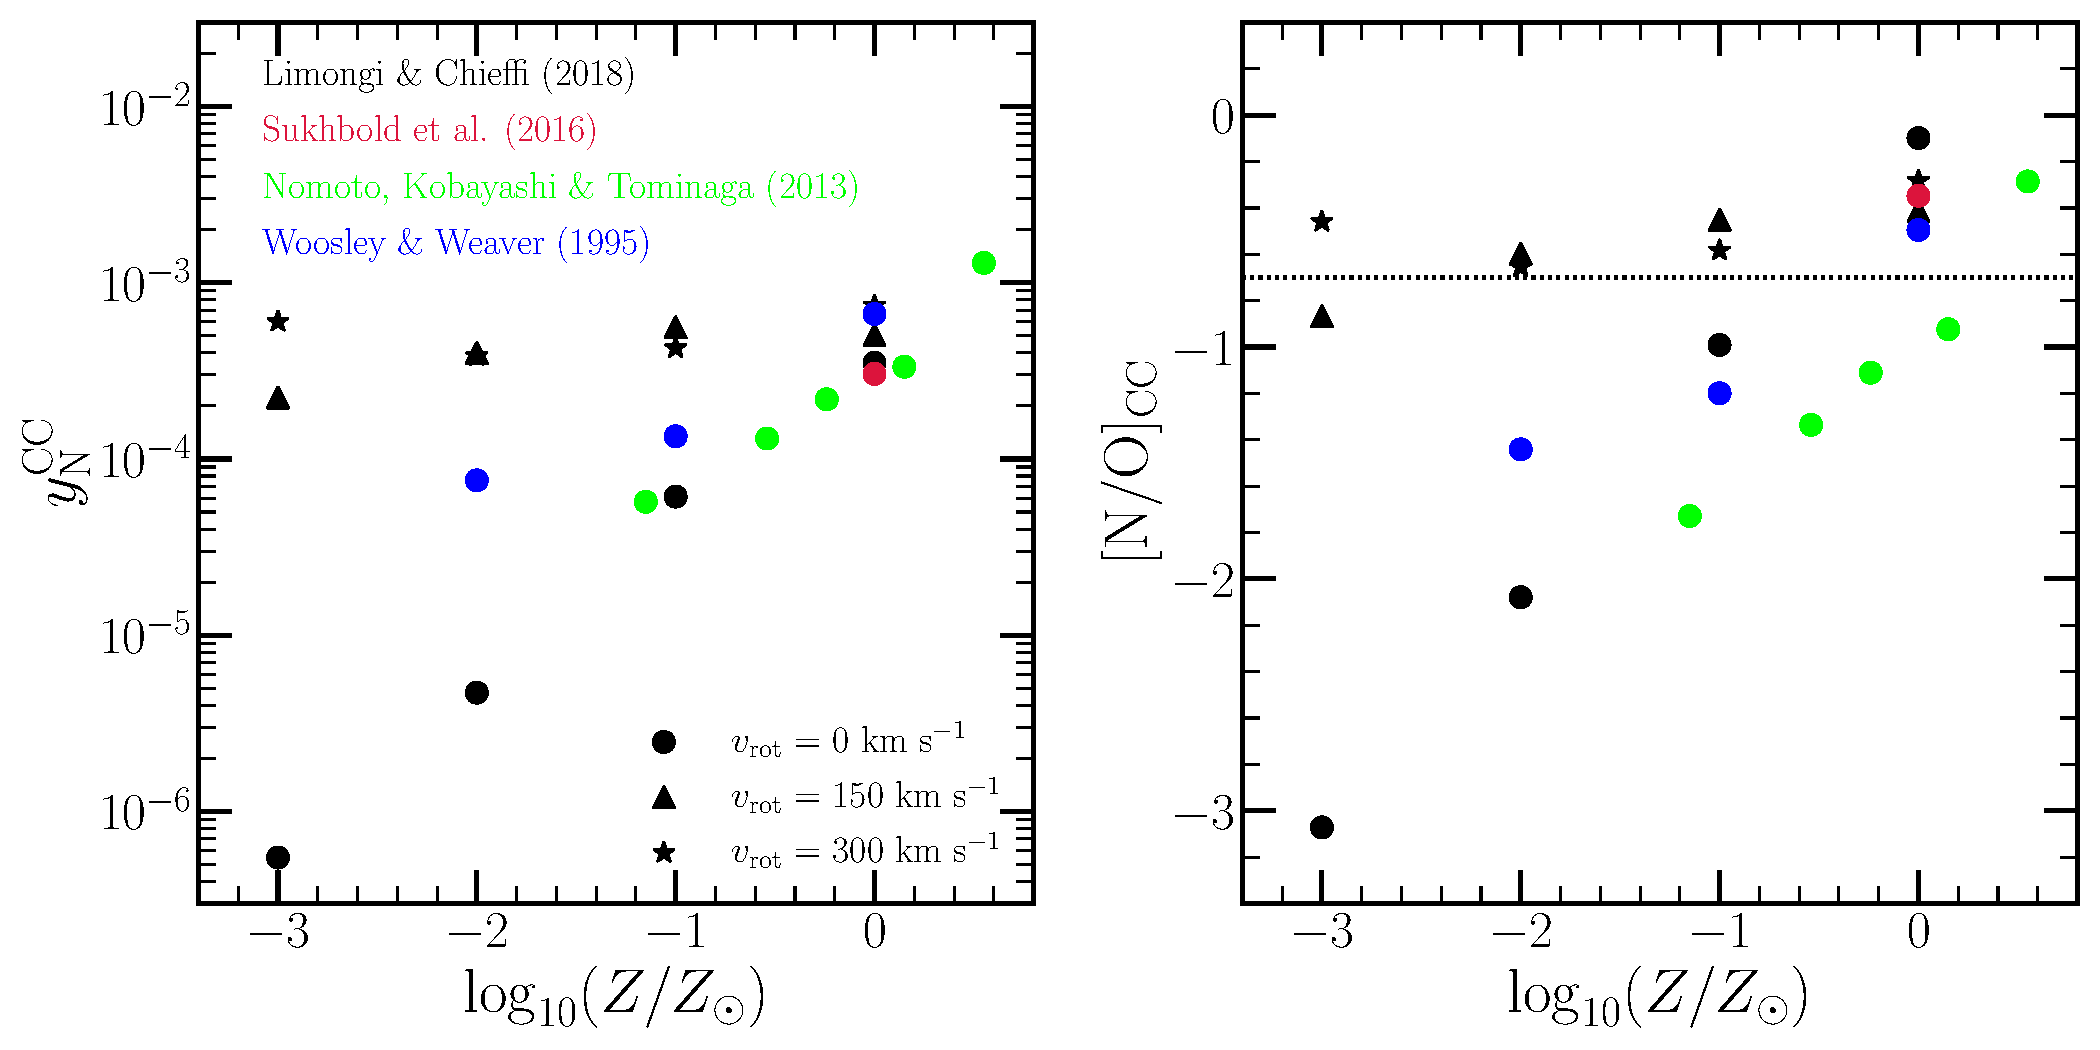
\includegraphics[scale = 0.5]{n_cc_yields.pdf} 
\caption{
\textbf{Left}: IMF-averaged CCSN yields of N calculated 
using~\vice's~\texttt{vice.yields.ccsne.fractional} function with the tables 
published by~\citet[][blue]{Woosley1995},~\citet*[][green]{Nomoto2013}, 
\citet[][red]{Sukhbold2016}, and~\citet[][black]{Limongi2018}. 
All studies report yields for non-rotating progenitors only with the exception 
of~\citet{Limongi2018}, who also report yields for progenitor rotational 
velocities of 150 (triangles) and 300 km/s (stars). 
\textbf{Right}: The~\no~ratio predicted by each of the explosion models in 
the left-hand panel, under the same colour-coding and marker scheme. 
We mark the position of~\no~= $-0.7$ with a black dotted line, the value 
roughly suggested by the observations of low-metallicity systems highlighted in 
Fig.~\ref{fig:no_oh_observed}. 
}
\label{fig:n_cc_yields} 
\end{figure*} 

\begin{itemize} 
	\item In~\vice, CCSN nucleosynthetic products are approximated to be 
	produced instantaneously following an episode of star formation; this is a 
	valid approximation due to how short the lives of massive stars are 
	compared to the relevant timescales for GCE. 
	The yield is the constant of proportionality between the CCSN production 
	rate and the SFR: 
	\begin{equation} 
	\dot{M}_\text{X}^\text{CC} = y_\text{X}^\text{CC}\dot{M}_\star. 
	\end{equation} 

	\item At low [O/H]\footnote{
		We follow the standard notation where 
		[X/Y]~$\equiv \log_{10}(X/Y) - \log_{10}(X/Y)_\odot$. 
	}, the mean~\no~is near~$\sim$-0.7 (see Fig.~\ref{fig:no_oh_observed}). 
	Since the AGB star yields of N are believed to increase with metallicity 
	(e.g.,~\cristallo;~\ventura), this is likely the regime in which N yields 
	are dominated by CCSN enrichment. 
	We therefore take~\no\subcc~$\approx -0.7$ empirically. 

	\item Based on the definition of the abundance ratio [X/Y], we can relate 
	the CCSN yields of N and O to one another given this result: 
	\begin{subequations}\begin{align} 
	\text{[N/O]}\subcc &= 
	\log_{10}\left(\frac{y_\text{N}^\text{CC}}{y_\text{O}^\text{CC}}\right) - 
	\log_{10}\left(\frac{Z_{\text{N},\odot}}{Z_{\text{O},\odot}}\right) 
	\label{eq:no_cc}
	\\ 
	y_\text{N}^\text{CC} &= 
	y_\text{O}^\text{CC} 10^{\no\subcc} 
	\left(\frac{Z_{\text{N},\odot}}{Z_{\text{O},\odot}}\right), 
	\end{align}\end{subequations} 
	where~$Z_{\text{X},\odot}$ is the abundance by mass of some element X in 
	the sun. 

	\item Taking~$Z_{\text{N},\odot} = 6.91\times10^{-4}$ 
	and~$Z_{\text{O},\odot} = 5.7\times10^{-3}$ based on the solar photospheric 
	abundances of~\citet{Asplund2009} and our value of~$y_\text{O}^\text{CC}$ = 
	0.015 yields~$y_\text{N}^\text{CC} = 3.6\times10^{-4}$, which we adopt as 
	our fiducial CCSN yield of N. 
	We mark this value with a horizontal dotted line in the left hand panel 
	of Fig.~\ref{fig:n_cc_yields}. 
	We discuss the sloped dotted line in that panel in the context of some of 
	our AGB star yield models in~\S~\ref{sec:results:yields}. 

	\item Can we understand this value with theoretically predicted N yields? 
	To address this, we compute IMF-averaged net yields of N using~\vice's 
	\texttt{vice.yields.ccsne.fractional} function assuming 
	a~\citet{Kroupa2001} IMF; for details, we refer readers to~\S~4 
	of~\citet{Griffith2021} and the~\vice~science documentation.\footnote{
		\url{https://vice-astro.readthedocs.io/en/latest/science_documentation/yields/index.html} 
	} 
	The left panel of Fig.~\ref{fig:n_cc_yields} plots the results as a 
	function of progenitor metallicity predicted by the~\citet{Woosley1995}, 
	\citet{Nomoto2013},~\citet{Sukhbold2016}, and~\citet{Limongi2018} tables. 

	% \item The left panel of Fig.~\ref{fig:n_cc_yields} plots the IMF-averaged 
	% CCSN yields of N as predicted by~\citet{Woosley1995},~\citet{Nomoto2013}, 
	% \citet{Sukhbold2016}, and~\citet{Limongi2018}. 
	%  using~\vice's~\texttt{vice.yields.ccsne.fractional} 
	% function assuming a~\citet{Kroupa2001} IMF 

	% These values, computed using~\vice's~\texttt{vice.yields.ccsne.fractional} 
	% function, describe the fractional net yield of an element X given by: 
	% \begin{equation} 
	% y_\text{X}^\text{CC} = \ddfrac{
	% 	\int_{8~\msun}^u (E(m)m_\text{X} + w_\text{X} - Z_\text{X,prog}m)
	% 	\frac{dN}{dm} dm 
	% }{
	% 	\int_l^u m\frac{dN}{dm} dm 
	% }, 
	% \end{equation} 
	% where~$m_\text{X}$ is the total mass of the element X in the supernova 
	% ejecta of a star of initial mass~$m$,~$w_\text{X}$ is the wind yield, 
	% $Z_\text{X,prog}$ is the initial abundance by mass of the element X in the 
	% star,~$E(m)$ is a function describing whether or not the star explodes as a 
	% supernova, and~$dN/dm$ is the adopted stellar IMF, for which we take 
	% the~\citet{Kroupa2001} form throughout this paper. 
	% These yields are fractional in that they're in units of the progenitor 
	% stellar population's mass (i.e. if~$y_\text{X}^\text{CC}$ = 0.01, a 
	% hypothetical 100~\msun~cluster would produce 1~\msun of X), and they're net 
	% rather than gross in that they quantify only the newly produced mass. 
	% The lower bound of the integral in the numerator, taken to be 8~\msun~here, 
	% simply corresponds to the minimum initial mass for a CCSN event, where the 
	% remaining bounds are simply the lower and upper mass bounds of star 
	% formation, for which we adopt~$l = 0.08$~\msun and~$u = 100$~\msun. 
	% For further details, we refer readers to~\S~4 of~\citet{Griffith2021} and 
	% the~\vice~science docuementation.\footnote{
	% 	\url{https://vice-astro.readthedocs.io/en/latest/science_documentation/yields/index.html} 
	% } 

	\item Only~\citet{Limongi2018} report yields for progenitors with a 
	non-zero rotational velocity, and these are the only values consistent 
	with~$y_\text{N}^\text{CC} = 3.6\times10^{-4}$ at low metallicity. 
	For non-rotating progentiors, every study investigated here can reproduce 
	approximately this value at solar metallicity only, with the predictions at 
	lower~$Z$ falling short of the empirical value, in some cases by orders of 
	magnitude. 

	\item It is unsurprising that~$y_\text{N}^\text{CC}$ is so dependent on the 
	rotational velocity at low metallicity. 
	$y_\text{N}^\text{CC}$ is itself highly uncertain at 
	low~$Z$~\citep{Heger2010}, but most of the N production in CCSN progenitors 
	occurs via the CNO cycle processing C and O isotopes into~\Nfourteen. 
	With few C and O seed nuclei at low~$Z$, production of~\Nfourteen~is 
	difficult. 
	Rotationally induced mixing, also a highly uncertain process 
	\citep{Zahn1992, Maeder1998, Lagarde2012}, could transport newly produced 
	C and O into the hydrogen burning shell of the CCSN progenitor, 
	facilitating N production (\citealp{Frischknecht2016}; see also discussion 
	in~\S~4.2 of~\citealp{Andrews2017}). 
	For this reason, N yields at low metallicity are highly sensitive to the 
	assumptions about mixing. 

	\item In the right-hand panel of Fig.~\ref{fig:n_cc_yields}, we make use of 
	equation~\refp{eq:no_cc} to compare the~\no~ratios predicted by these 
	studies; the horizontal black dashed line denotes~\no\subcc~$= -0.07$, the 
	empirical value taken from Fig.~\ref{fig:no_oh_observed}. 
	The fact that the points follow similar trends between the two panels is a 
	consequence of the fact that these studies predict relatively 
	metallicity-independent O yields. 

	\item Again, only the rotating models of~\citet{Limongi2018} are able to 
	reproduce this value at low metallicity. 
	At solar metallicity the supernova models predict a higher~\no\subcc, but 
	our value of~\no\subcc~is taken at low metallicity, so that is the 
	most relevant comparison. 
\end{itemize} 

\subsubsection{Asymptotic Giant Branch Stars} 
\label{sec:methods:yields:agb} 

\begin{figure*} 
\centering 
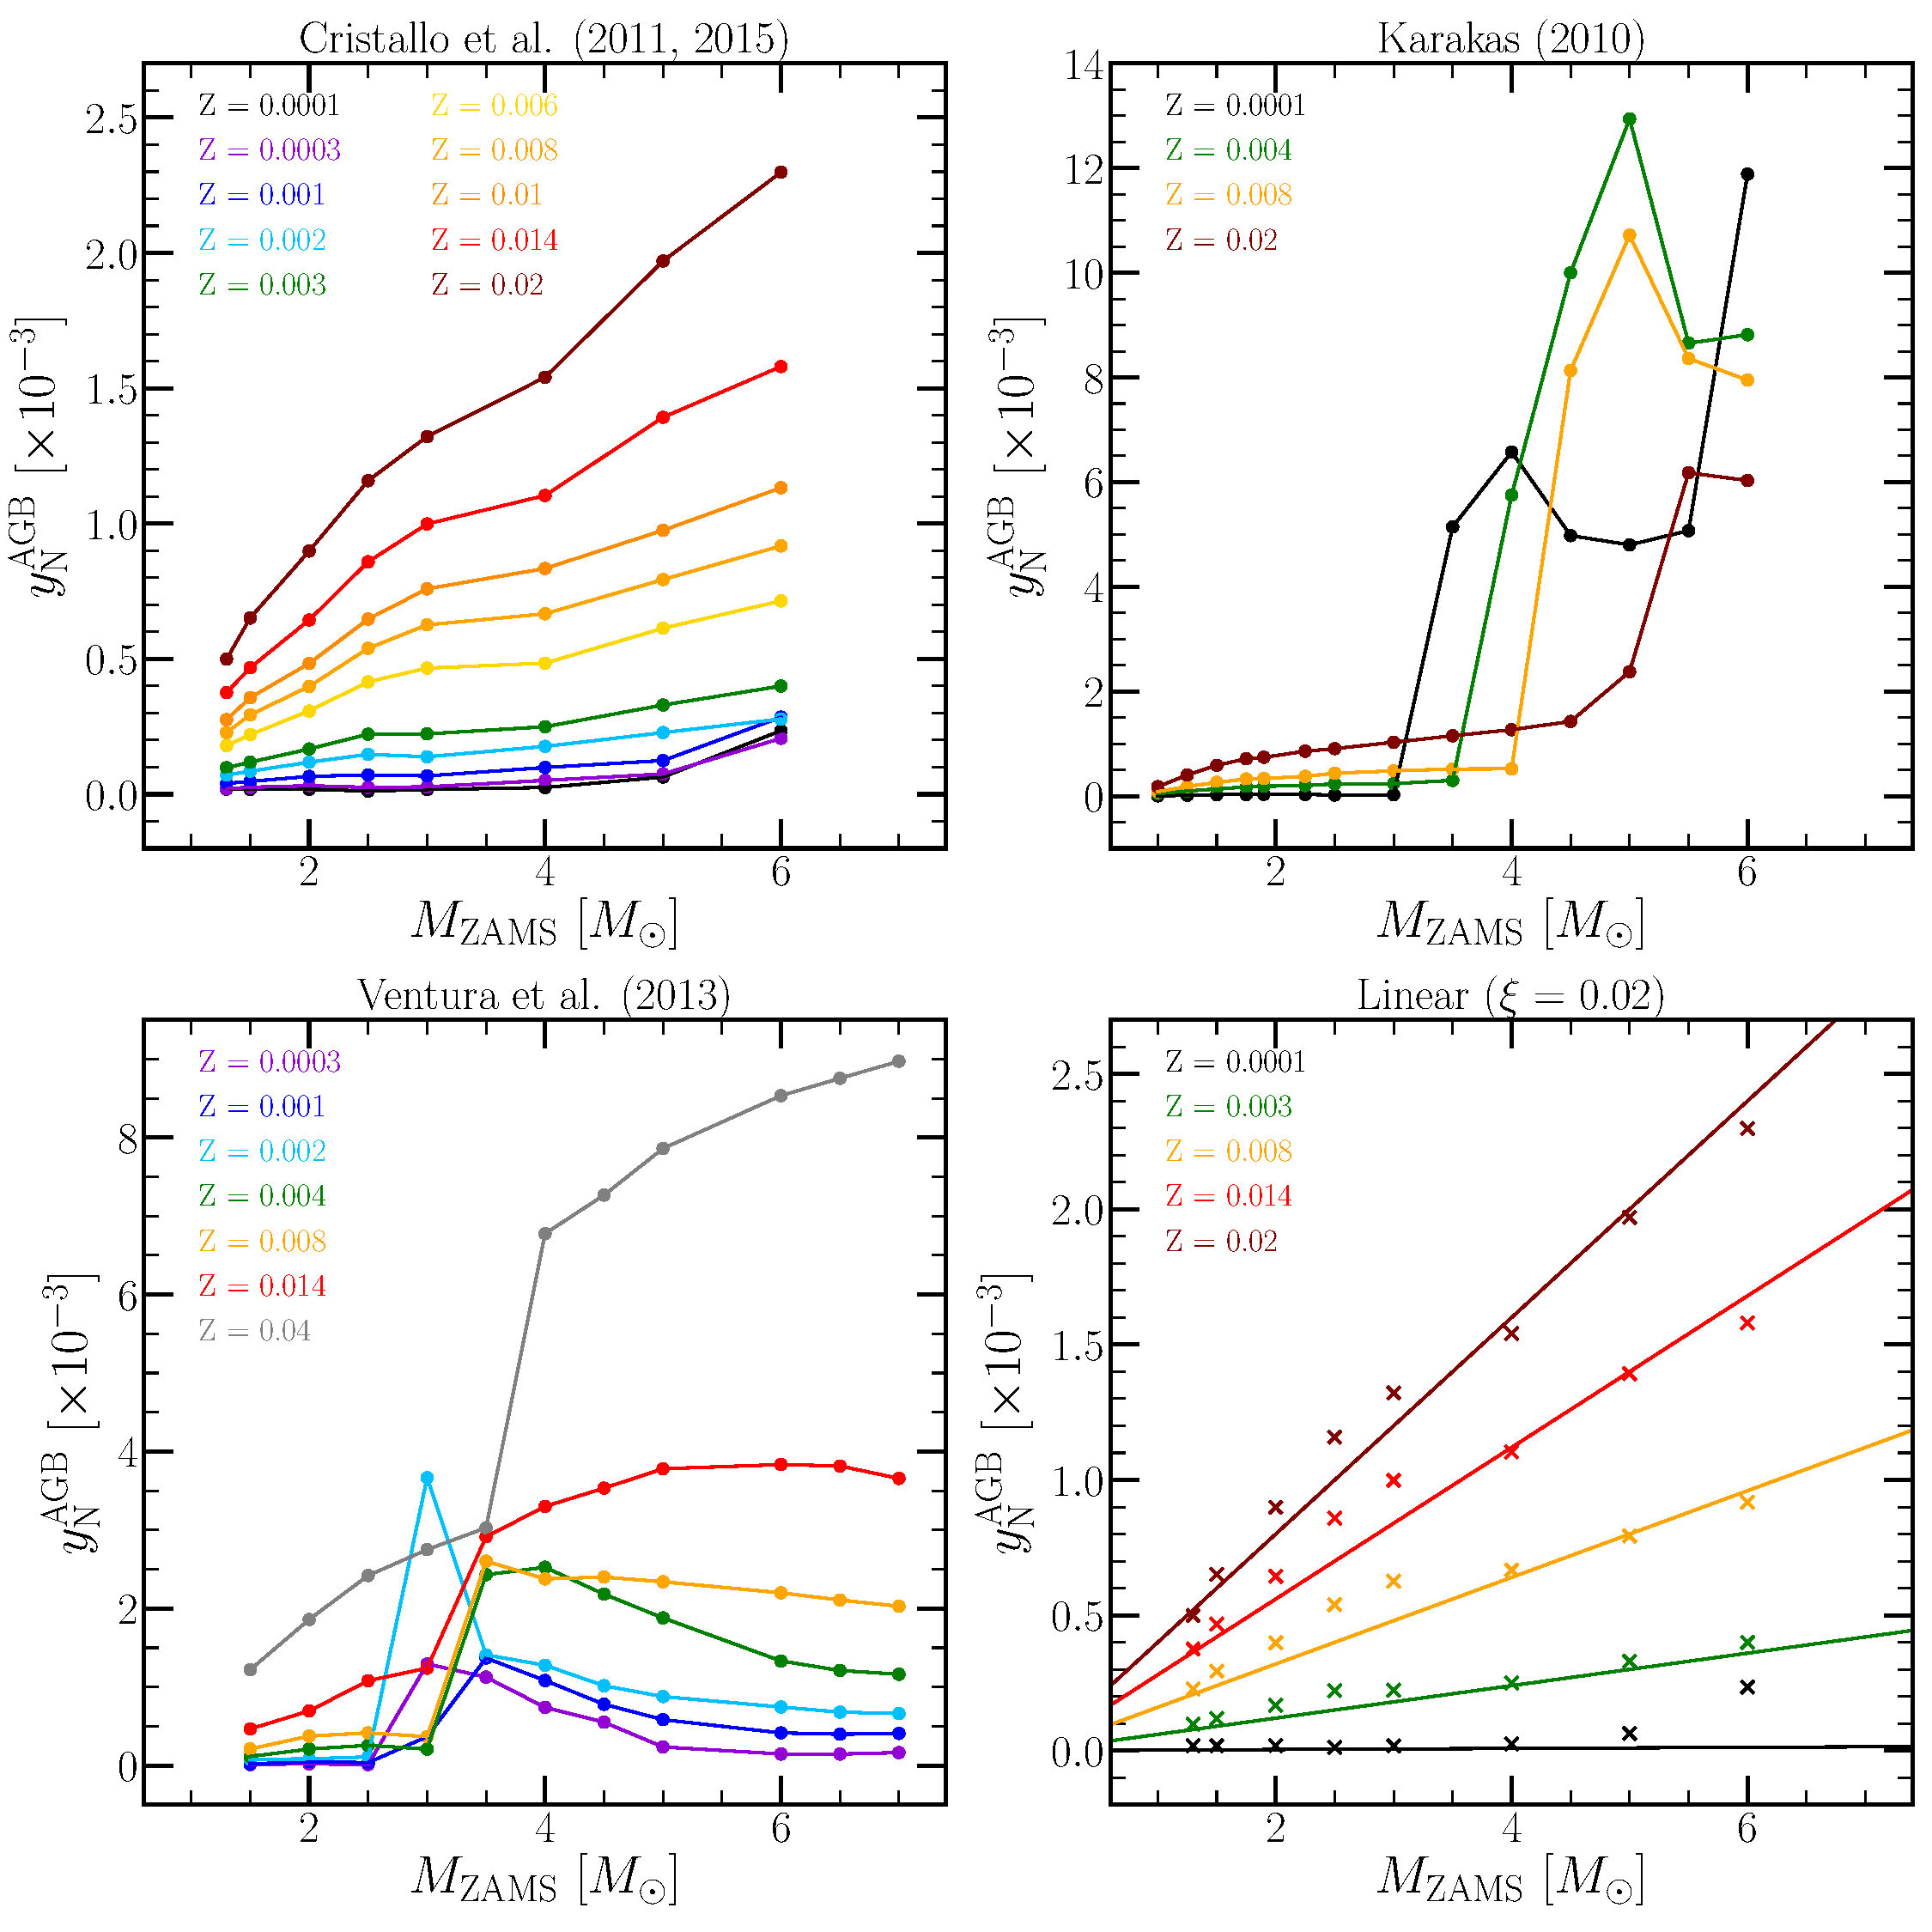
\includegraphics[scale = 0.33]{agb_yield_models.pdf} 
\caption{
The fractional yields of N from AGB stars~$y_\text{N}^\text{AGB}$ as a function 
of progenitor ZAMS mass and birth metallicity~$Z$ as reported 
by~\citet{Karakas2010} (upper left),~\citet{Karakas2016} and~\citet{Karakas2018} 
(upper middle),~\citet{Cristallo2011, Cristallo2015} (lower left), 
and~\citet{Ventura2013} (lower middle). 
In the lower right panel, we show the yields predicted by our linear model 
(colored lines; see discussion in~\S~X) in comparison to 
the~\citet{Cristallo2011, Cristallo2015} predictions (colored X's). 
}
\label{fig:agb_yield_models} 
\end{figure*} 

\begin{itemize} 
	\item In the present paper, we're interested in the question of how 
	well the ``off the shelf'' AGB star yield models for N can reproduce the 
	observed [N/O]-[O/H] relation. 

	\item {[As discussed in~\S~\ref{sec:intro},]} the majority of nitrogen 
	production occurs through the CNO cycle, the slowest component of which is 
	the~\Nfourteen(p,$\gamma$)\Ofifteen~reaction which produces a bottleneck, 
	effectively turning all of the different C, N, and O isotopes 
	into~\Nfourteen. 

	\item Similar to the SN yields (see discussion above), these are defined as 
	fractional net yields in that they quantify only the newly produced N in 
	the AGB star ejecta in units of its ZAMS mass. 
	For a yield~$y_\text{N}^\text{AGB}(M_\star, Z_\star)$, the actual mass 
	yield is then given by~$M_\star y_\text{N}^\text{AGB}(M_\star, Z_\star)$. 
	AGB star enrichment proceeds as it does in~\citet{Johnson2020} under the 
	caveat that the yield is placed in the~$\delta\rgal$ = 100 pc ring that a 
	stellar population is in at a given time. 
	In short,~\vice~implements an algorithm which calculates the mass in dying 
	stars from each previous star formation event (i.e. timestep), and the ZAMS 
	mass required to calculate the yield comes from a mass-lifetime 
	relation~\citep*[e.g.][]{Hurley2000}. 

	\item In the present paper, we make use of four previously published yields 
	calculated from stellar evolution models on a table of progenitor masses 
	and metallicities. 
	Two of these yield sets are already built in~\vice: 
	\begin{itemize} 
		\item The default set of yields is published in~\citet{Cristallo2011, 
		Cristallo2015} (hereafter~\cristallo). 
		We illustrate these yields as a function of ZAMS mass for the available 
		metallicities in the lower left panel of 
		Fig.~\ref{fig:agb_yield_models}. 
		This is the most comprehensive set of yields in~\vice~in that it 
		includes tables for all elements built into the code and is sampled at 
		the most metallicities. 

		\item The~\citet[][hereafter~\karakasten]{Karakas2010} is plotted in 
		the upper left panel of Fig.~\ref{fig:agb_yield_models}. 
	\end{itemize} 
	With this paper we build in the following additional sets of AGB star yield 
	tables: 
	\begin{itemize} 
		\item The~\citet[][hereafter~\ventura]{Ventura2013} yields are 
		illustrated in the bottom middle panel of 
		Fig.~\ref{fig:agb_yield_models}. 

		\item We combine the yields published in~\citet{Karakas2016} at~$Z$ = 
		0.007, 0.014, and 0.03 with those published in~\citet{Karakas2018} 
		at~$Z$ = 0.0028; we hereafter refer to these tables as the~\karakas~set 
		of yields. 
		We plot them in the upper middle panel of 
		Fig.~\ref{fig:agb_yield_models}. 
	\end{itemize} 

	\item \vice~also allows users to construct their own functions of 
	progenitor mass and metallicity to describe the AGB star yield. 
	As an additional test, we construct a model in which the yield is linearly 
	proportional to both progenitor ZAMS mass and metallicity according to: 
	\begin{equation} 
	y_\text{N}^\text{AGB} = \xi\left(\frac{M}{M_\odot}\right) 
	\left(\frac{Z}{Z_\odot}\right) 
	\label{eq:linear_yield} 
	\end{equation} 
	We illustrate this model in the lower right panel of 
	Fig.~\ref{fig:agb_yield_models} for~$\xi = 3\times10^{-4}$. 
	We compare this model to the~\cristallo~yields by including the colored X's 
	on this panel. 
	In general, the two yield models agree rather well. 
\end{itemize}

\begin{figure*} 
\centering 
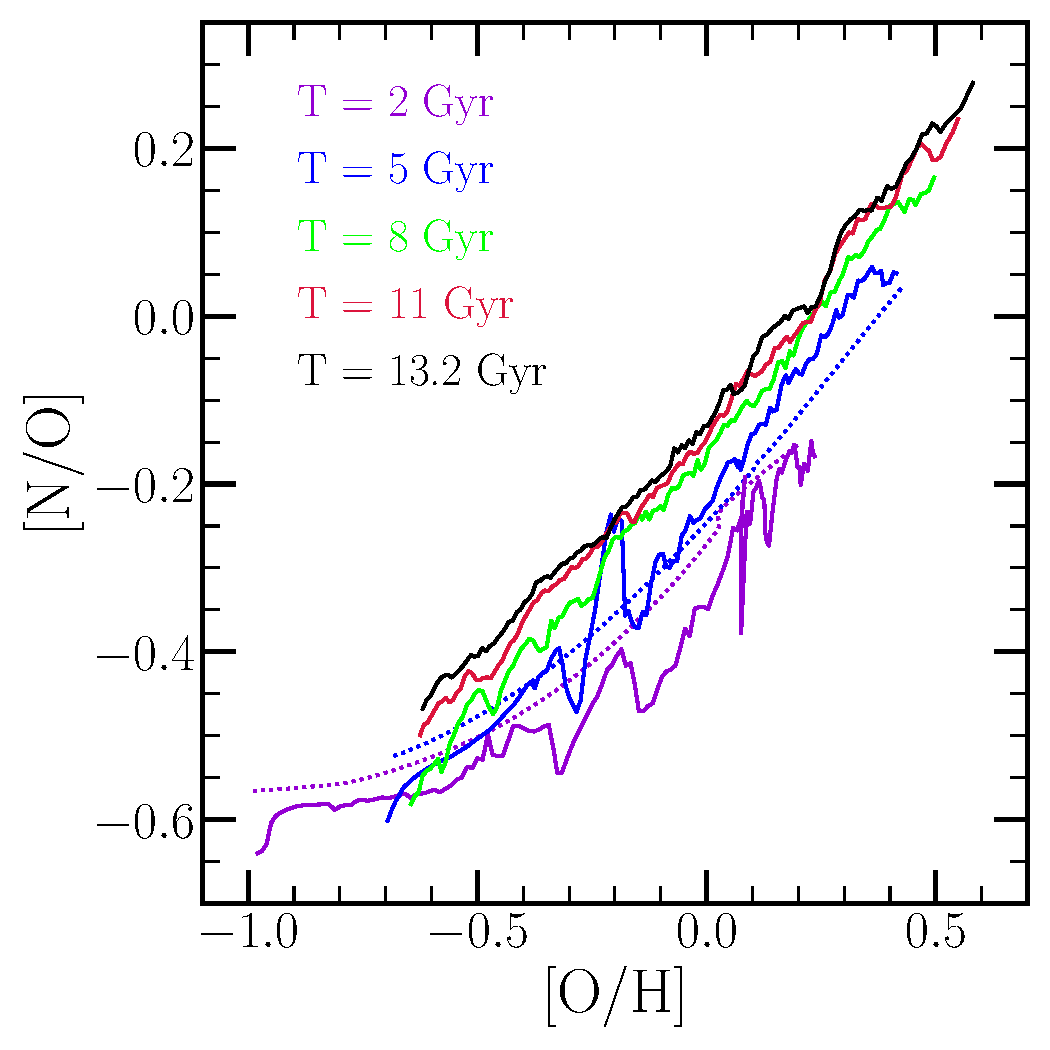
\includegraphics[scale = 0.3]{no_oh_timeevol.pdf} 
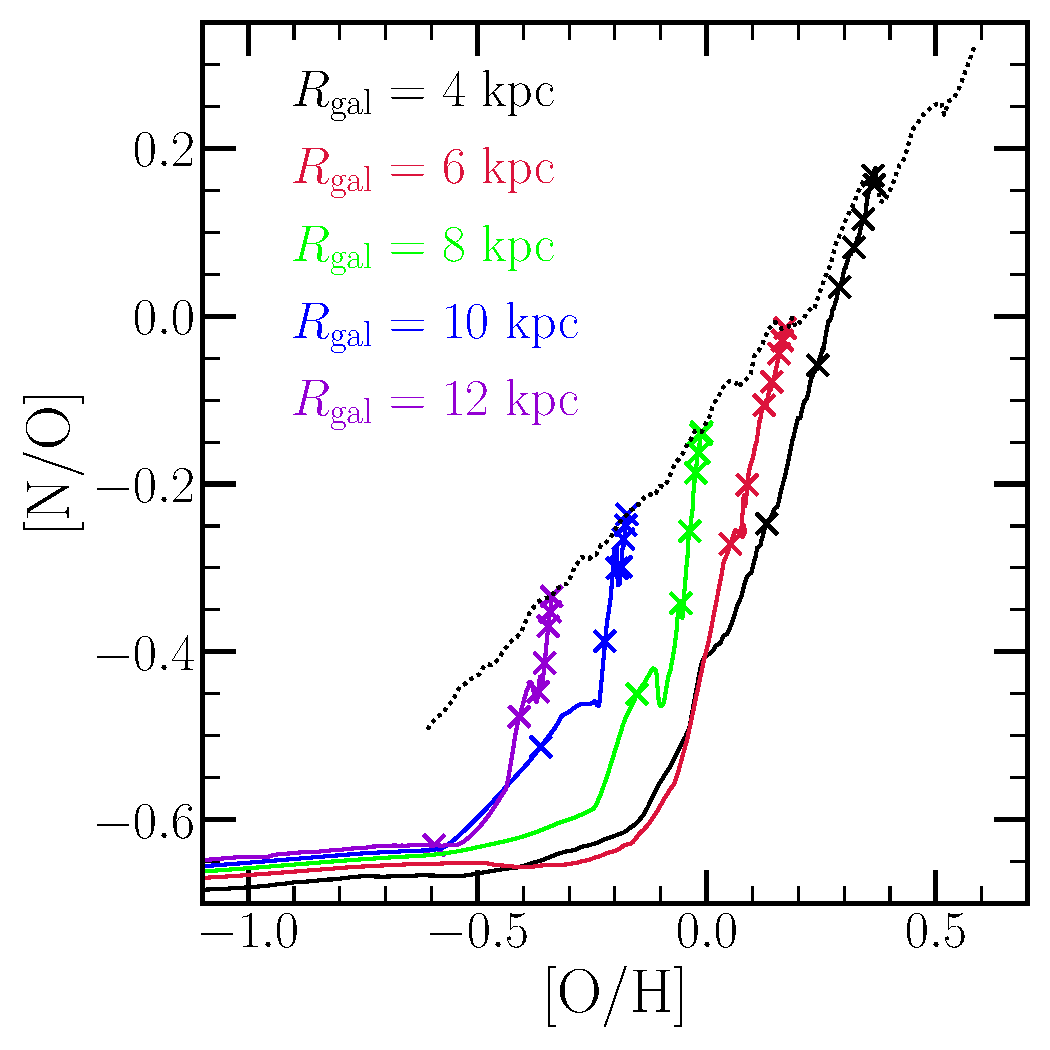
\includegraphics[scale = 0.3]{no_oh_superposition.pdf} 
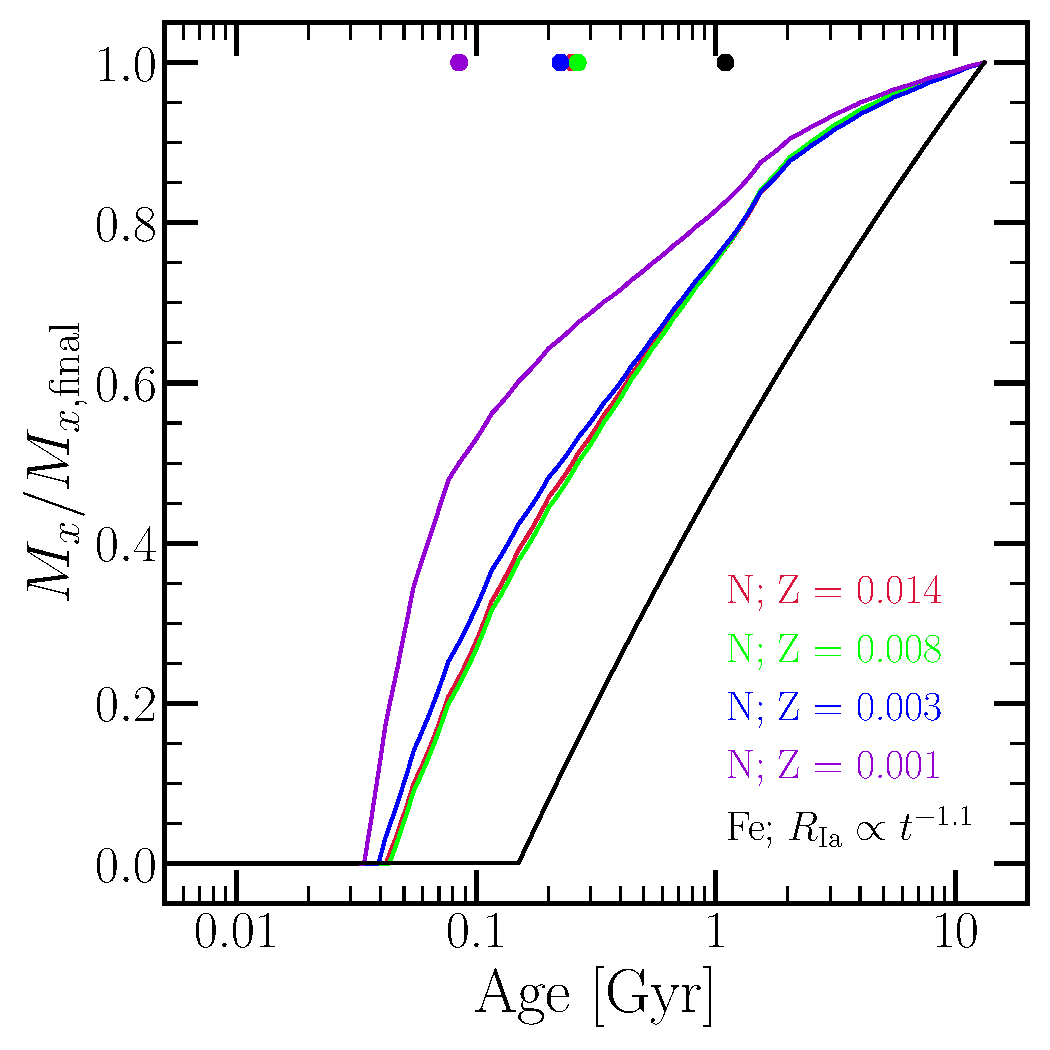
\includegraphics[scale = 0.3]{ssp_production.pdf} 
\caption{
\textbf{Left}: The gas-phase [N/O]-[O/H] relation parameterized by radius at 
various snapshots (solid coloured lines) in our fiducial model with 
the~\cristallo~yields. 
Dotted lines denote the resulting relation at~$T$ = 2 and 5 Gyr in the model 
where we neglect stellar migration. 
\textbf{Middle}: The gas-phase [N/O]-[O/H] relation parameterized by time at 
fixed radius (solid coloured lines) in the fiducial model. 
X's denote the abundances at~$T$ = 2, 4, 6, 8, 10, 12, and 13.2 Gyr (the 
present day) at these radii. 
The dotted line is the same as the solid black line in the left hand panel. 
\textbf{Right}: The net mass of N produced by AGB stars from a single stellar 
population assuming four initial metallicities and the~\cristallo~yields 
(coloured lines). 
The black line denotes the same for Fe assuming the~$t^{-1.1}$ power-law delay 
time distribution adopted in our models. 
All values are normalized to the total mass produced at an age of 13.2 Gyr. 
Points at the top of the panel denote the ages at which 50\% of the total mass 
yield has been produced. 
} 
\label{fig:no_oh_timeevol_ssp} 
\end{figure*} 

\begin{itemize} 
	\item Despite reporting values of the same physical quantities, the N 
	yields reported by each of these studies show substantial differences 
	between one another. 
	Unfortunately, a direct comparison between AGB star yield tables is 
	difficult, because each study employs different assumptions for mass loss, 
	convection and covective boundaries within the star, and nuclear reaction 
	networks, all of which have a significant impact on stellar evolution and 
	consequently the predicted abundances. 
	However, the two most important physical processes in determining AGB star 
	yields of all the CNO species is third dredge up (TDU) and hot bottom 
	burning (HBB), and some of the differences between these yield sets can be 
	understood through the interaction between the two. 
	\begin{itemize} 
		\item TDU refers to the repeated penetrations of the convective 
		envelope into the hydrogen depleted core during the thermal pulses 
		associated with AGB star evolution. 
		This process doesn't affect N abundances much, but replenishes the 
		outer layers of the star with C and O. 
		In low mass AGB stars, the main source of free neutrons is the 
		\Cthirteen($\alpha$,n)\Osixteen~reaction, which can occur at 
		substantial rates when C is mixed with the He-rich shell during each 
		TDU episode. 

		\item HBB refers to the activation of proton captures at the base of 
		the convective envelope, which activates the CNO cycle, producing large 
		amounts of~\Nfourteen at the expense of C and O. HBB requires a higher 
		mass AGB star progenitor ($\sim$4 - 5~\msun at Z$_\odot$) than TDU 
		($\sim$2 - 2.5~\msun at Z$_\odot$), but the minimum mass for both 
		decreases at lower metallicity. 

		\item The most efficient N production occurs when both TDU and HBB 
		occur within an AGB star, because each replenishment of C and O 
		isotopes from the core adds new seed nuclei for the CNO cycle when HBB 
		is active. 
		This is the reason for the substantial N production 
		above~$\sim$4~\msun~in the~\karakasten and~\karakas~models; in both 
		yield sets, every star that experiences HBB also experiences TDU. 
		Both TDU and HBB are more efficient at low metallicity (see discussion 
		in~\ventura). 
		In the case of TDU, each penetration of the convective envelope into 
		the H-depleted core is deeper because of the lower opacity. 
		For HBB, the base of the convective envelope is hotter, increasing the 
		rate of nuclear reactions relative to the higher~$Z$ models. 
		Though there are some exceptions evident in 
		Fig.~\ref{fig:agb_yield_models}, as a consequence the highest N yields 
		in the~\karakasten~and~\karakas~models are for low metallicity stars 
		above~$\sim$4~\msun. 

		\item This interaction between TDU and HBB is also the reason for the 
		increase in N yields in the~\ventura~tables near~$\sim$3~\msun. 
		Unlike the~\karakasten~and~\karakas~models, their stars experience 
		both TDU and HBB only in this narrow range in mass. 

		\item Of all of these yields taken from the literature, 
		the~\cristallo~sample shows the smoothest dependence on progenitor mass 
		and metallicity. 
		Unfortunately, ascertaining the exact cause of this difference between 
		the other yields explored here is difficult; relative to 
		the~\karakas~yields (see discussion in their~\S~5), 
		the~\cristallo~models have more mass loss, a~$\sim$10\% faster 
		triple-$\alpha$ reaction rate, weaker HBB, and fewer thermal pulses 
		overall. 
		Though their agreement is good below~$\lesssim$3~\msun, the fact that 
		HBB is weaker and fewer TDU episodes are experienced does however lend 
		a qualitative explanation into why the~\cristallo~yields are so much 
		smaller than the~\karakasten~and~\karakas~yields at higher masses. 
	\end{itemize} 

	\item In the interest of consistency, when we adopt a particular AGB star 
	yield model for N, we also adopt it for O and Fe. 
	However, the AGB star yields of these elements are negligible compared to 
	their supernova yields. 

\end{itemize} 

\end{document} 
